\section{Contemporary empirical dashboards}\label{sec:dashboards}

\subsection{Sources, competing criteria and training-origin design}
The real-data illustration uses the frozen NOAA Global Monitoring
Laboratory Mauna Loa monthly-mean atmospheric CO$_2$ concentrations
from January 1990 through September 2026 ($n=441$, last reported
value 426.07 ppm) \cite{noaa2026mlo}, and the monthly US
effective federal funds rate FEDFUNDS from January 2010 through
September 2026 ($n=201$, last reported value 3.75 percent)
\cite{fred2026fedfunds}. The FEDFUNDS observations are monthly
averages of daily effective rates, not seasonally adjusted. We
also repeat the CO$_2$ analysis on its last 120 observed months
to examine sensitivity to the estimation window. All raw data
and publisher vintages are frozen in the accompanying source
repository; neither dataset contains invented October 2026
observations.

At each difference order $d\in\{1,2,3,4\}$ we evaluate six
procedures: classical leave-one-out CV, GCV, AICc, BIC, a
Gaussian marginal profile likelihood criterion (MLE), and
user-controlled normalized smoothness $S=0.86$. The first five
criteria each minimize their own in-sample score over the
\emph{same} 29 candidate penalties obtained by inverting
the grid
\[
  \mathcal S=\{0.10+0.88j/28:j=0,\ldots,28\},\quad
  \lambda_j=S^{-1}(s_j).
\]
Thus, differences among those selections at a fixed $d$ and
$\mu$ do not arise from different candidate penalty grids.
The bounded grid cannot certify a global optimum, and an
optimum on its lowest or highest candidate is a \emph{grid
boundary} result. Controlled $S=0.86$ is a prescribed
smoothness level, \emph{not} a sixth optimization criterion.

\subsection{Reference difference mean and conditional likelihood}
We repeat the analysis under two specifications:
\[
  \mu_0=0,\qquad
  \widehat\mu_{d,\mathcal T}
  =\frac{1}{|\mathcal T|-d}
  \mathbf1^\top D_d y_{\mathcal T},
\]
where $\mathcal T$ is the \emph{available training window}
at the relevant origin. The second value depends on the
difference order and is not a universal drift parameter
shared across orders. For CV, GCV, AICc and BIC, we treat
the numeric $\widehat\mu_{d,\mathcal T}$ as \emph{fixed
conditional on that training sample} when scoring candidate
penalties. In particular the reported CV is not the exact
leave-one-out score for a procedure that re-estimates
$\mu$ in every deletion. The MLE panel uses the current
library's \texttt{mu="data"} plug-in: its Gaussian marginal
likelihood is profiled over variance conditional on this
reference mean, \emph{not jointly maximized over
$(\lambda,\mu)$}. For $\mu=0$ the same MLE criterion is
evaluated with that fixed value. All results report both
the numeric $\mu$ and the selected pair
$(\widehat\lambda,S(\widehat\lambda))$.

\subsection{Historical 12-month holdout dashboard}
We reserve the final 12 complete observed months of each
series. For every row/column combination, its reference mean,
penalty and PLS trend are fitted using the earlier training
segment \emph{only}. Rows correspond to $d=1,2,3,4$ and
columns to CV, GCV, AICc, BIC, MLE, and controlled
smoothness. Panel-level RMSE and MAE compare the resulting
12-month \emph{trend extrapolations} with the held-out raw
observations. The selected penalties and the numeric
plug-in means are recomputed when the origin changes.

\begin{figure}[p]
\centering
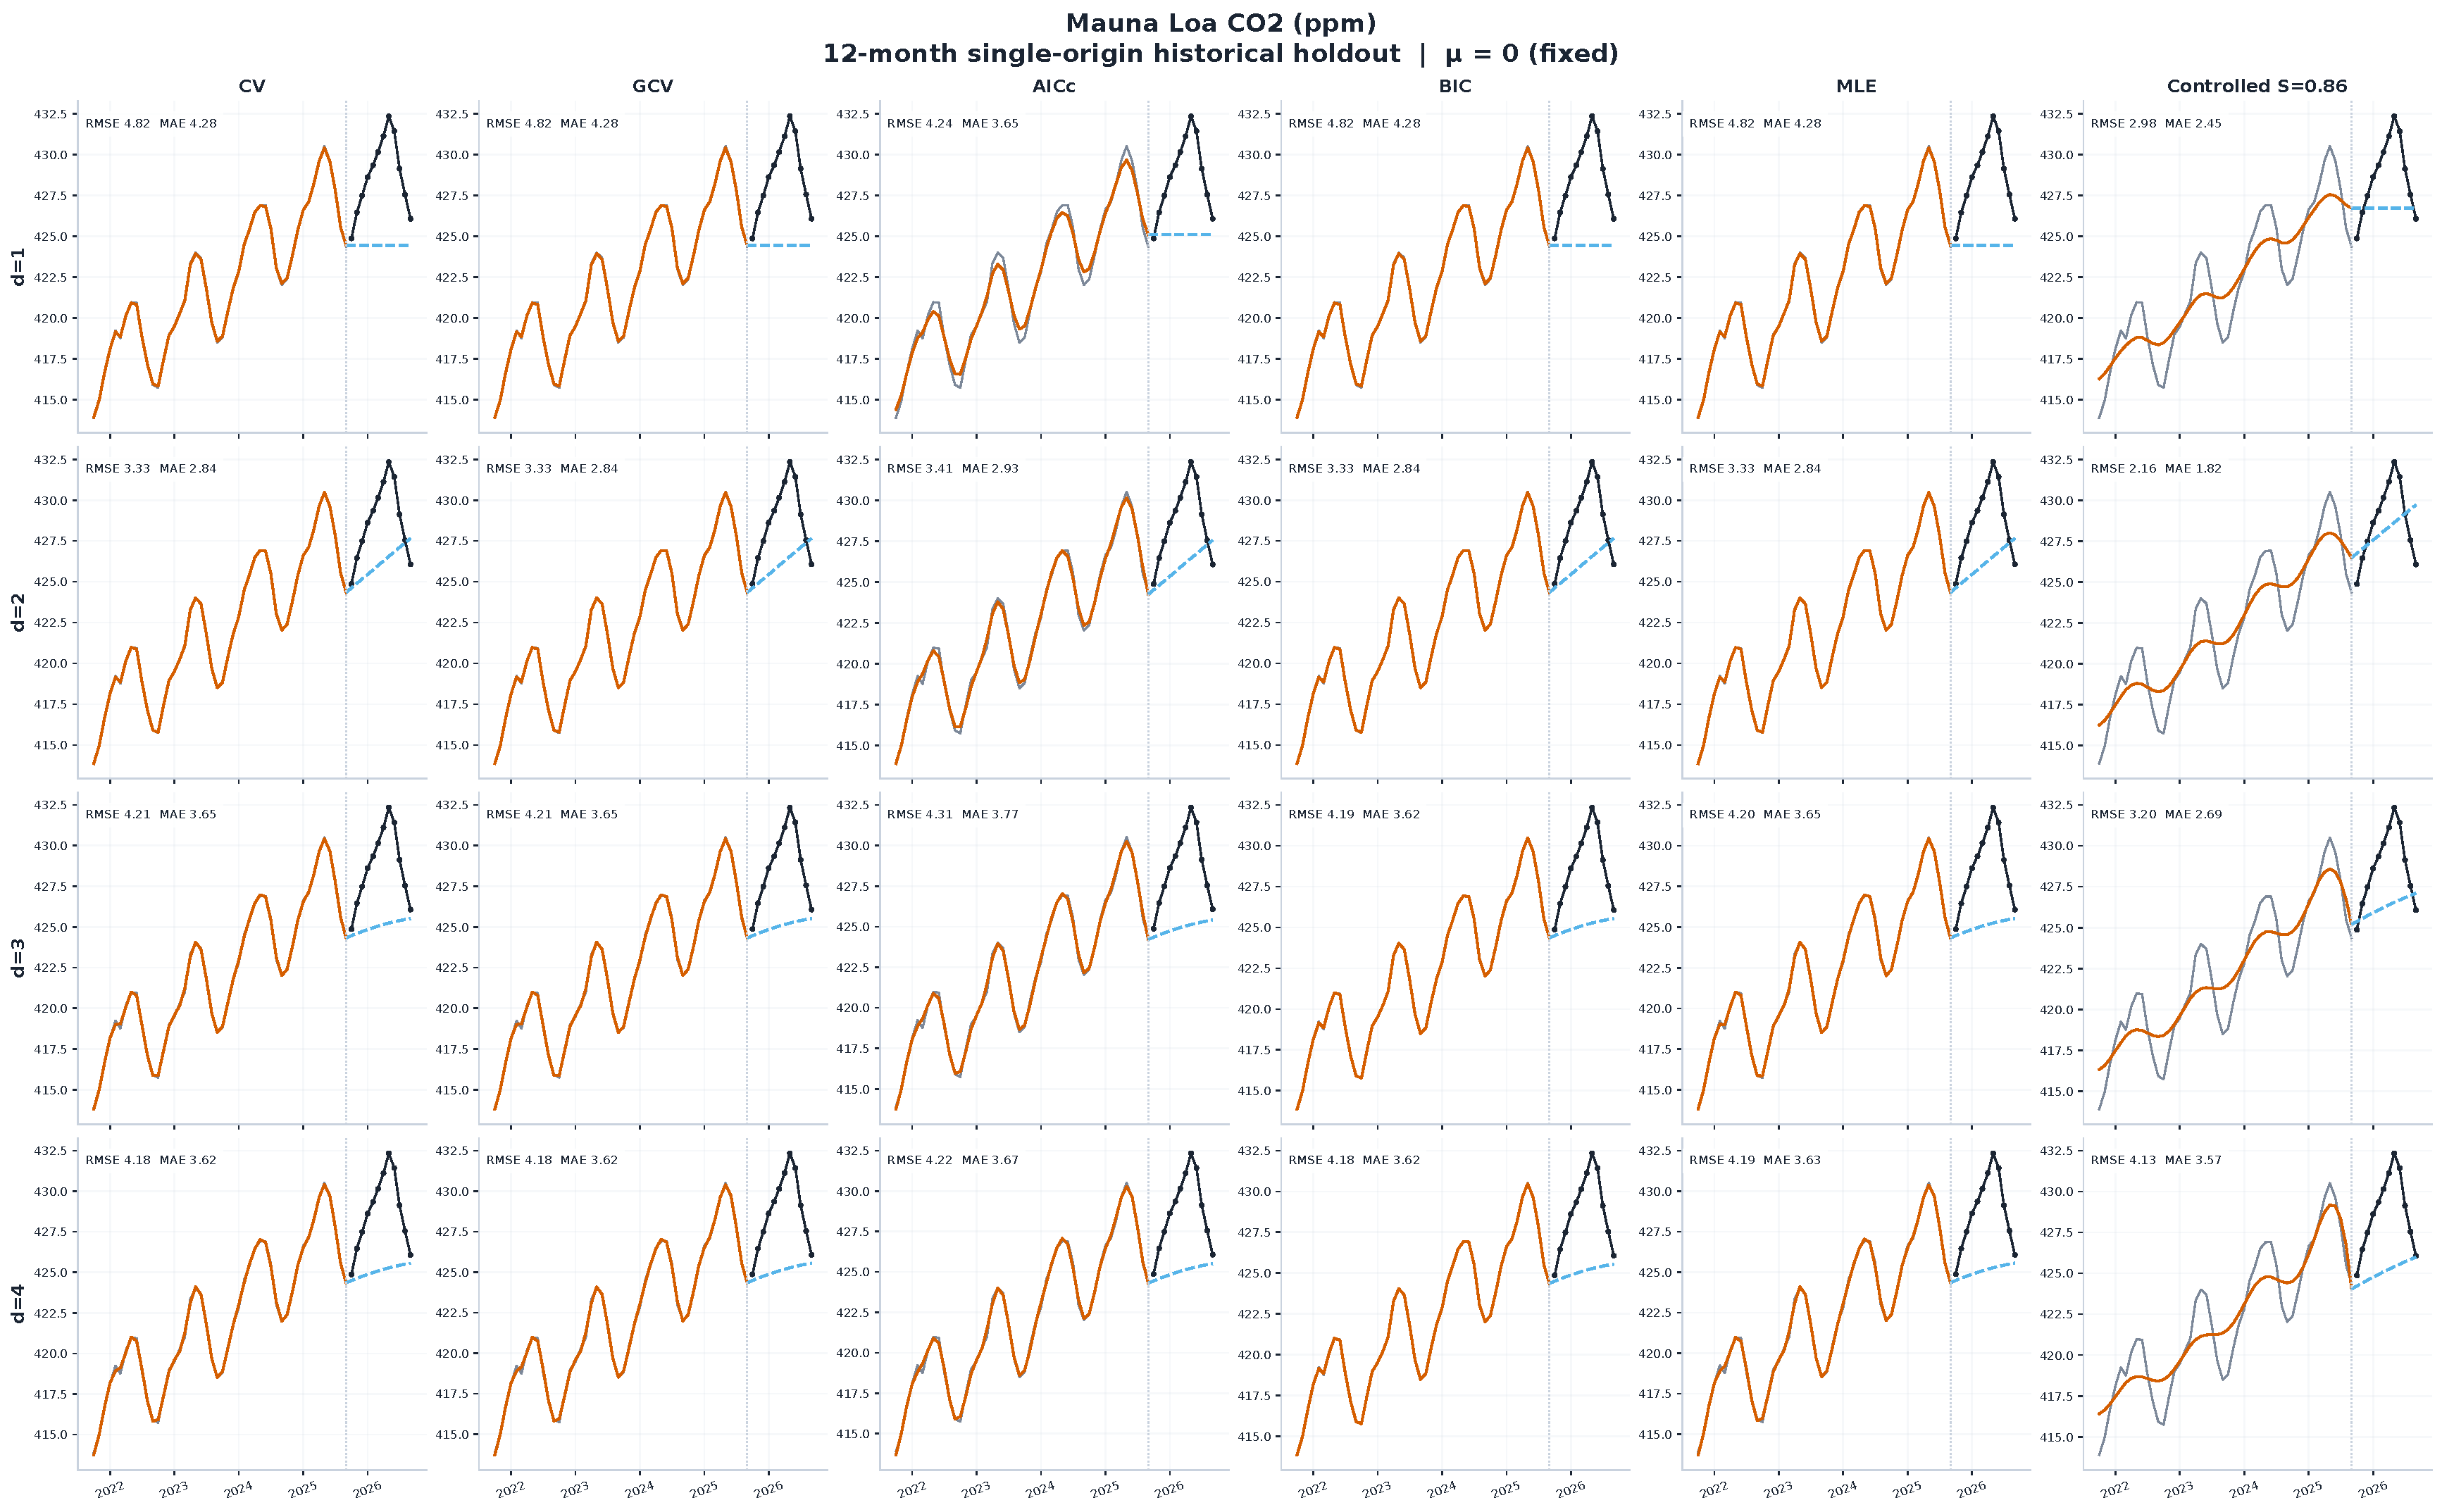
\includegraphics[width=\linewidth]{figures/co2_full_dashboard_holdout_mu_zero.pdf}
\caption{Mauna Loa CO$_2$ historical 12-month single-origin
holdout with fixed $\mu=0$. Rows are difference orders
$d=1,2,3,4$ and columns are CV, GCV, AICc, BIC, MLE,
and prescribed $S=0.86$. Gray curves represent observed
training data, blue curves are fitted historical PLS
trends, black markers are the held-out observations,
and dashed orange curves are 12-step extrapolations
constructed without knowledge of that holdout.
Full-resolution vector panels accompany the source code.
Scores are in-sample criteria; holdout losses measure
the extra extrapolation procedure, not a separately
specified stochastic forecast model.}
\label{fig:co2-holdout-dashboard}
\end{figure}

\subsection{Full-sample future trend extrapolation}
With the final data month included, we fit each smoother
again and extend the estimated trend for 12 future
calendar months (October 2026--September 2027).
The PLS estimator is two-sided on observed data; it does
\emph{not} intrinsically define future observations.
We therefore use an explicit tail rule: regress the last
up to 36 fitted monthly trend values on a locally centered
polynomial of degree $\min(d-1,2)$, shift that polynomial
to pass through the final fitted trend, and extrapolate
it one to 12 steps ahead. $d=1$ thereby produces a
constant continuation, $d=2$ a locally linear one, and
$d\ge3$ a quadratic continuation under the stated cap.
No future seasonality, innovations, or prediction
intervals are modelled.

\begin{figure}[p]
\centering
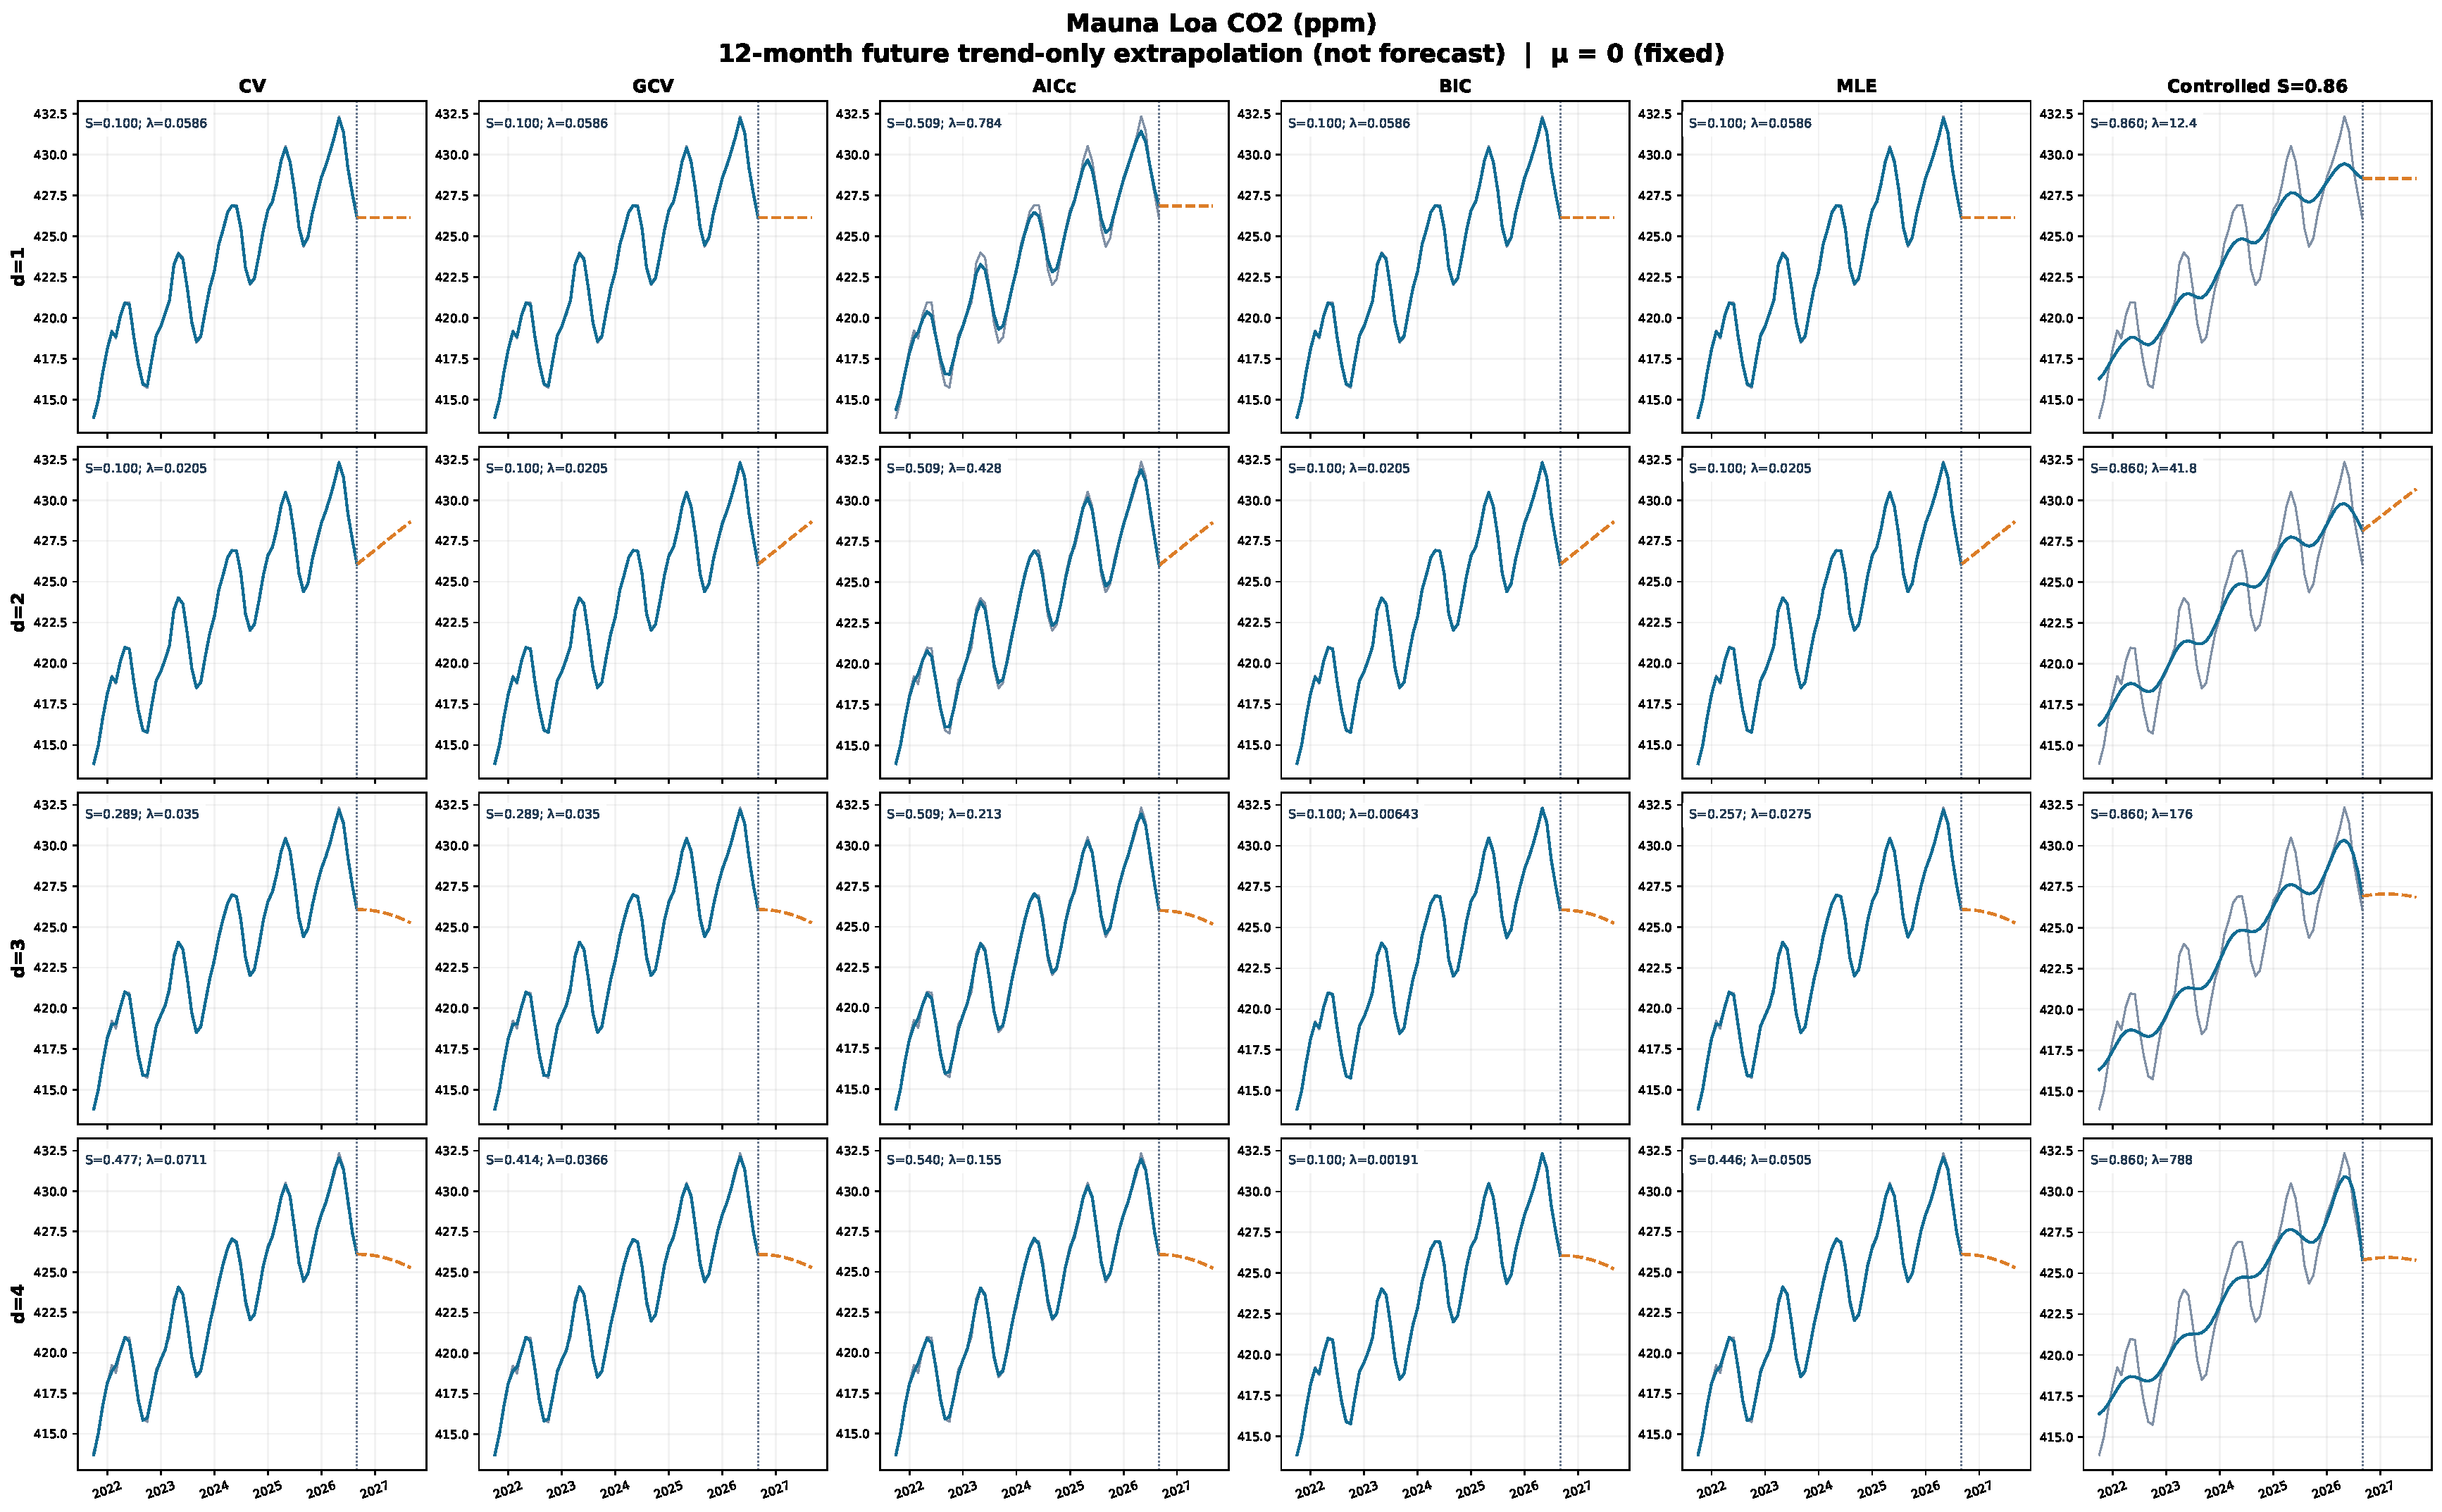
\includegraphics[width=\linewidth]{figures/co2_full_dashboard_future_mu_zero.pdf}
\caption{Full-sample Mauna Loa CO$_2$ trend extensions
under $\mu=0$ in the same $4\times6$ method/order layout.
Dashed segments lie \emph{beyond} the September 2026
observed-data cutoff and are descriptive anchored
polynomial extensions, not observed data, validated
stochastic forecasts, or confidence bands.}
\label{fig:co2-future-dashboard}
\end{figure}

\subsection{Smoothness, likelihood and holdout error}
Figure~\ref{fig:co2-selection-dashboard} reports the
selected raw penalty, its normalized smoothness,
and historical holdout RMSE and MAE across orders.
The penalty $\lambda$ and the normalized trace
coordinate $S(\lambda)$ describe \emph{the same
fit}, not competing estimates.
Unlike the penalty, a common target $S$ normalizes
the fraction of penalizable degrees of freedom across
$d$; it does not make the geometric trend shapes
or extrapolation rules equal. The MLE column differs
from CV/GCV/AICc/BIC through its probabilistic
profile-likelihood criterion; its numerical score is
not directly comparable with their objective values.

\begin{figure}[p]
\centering
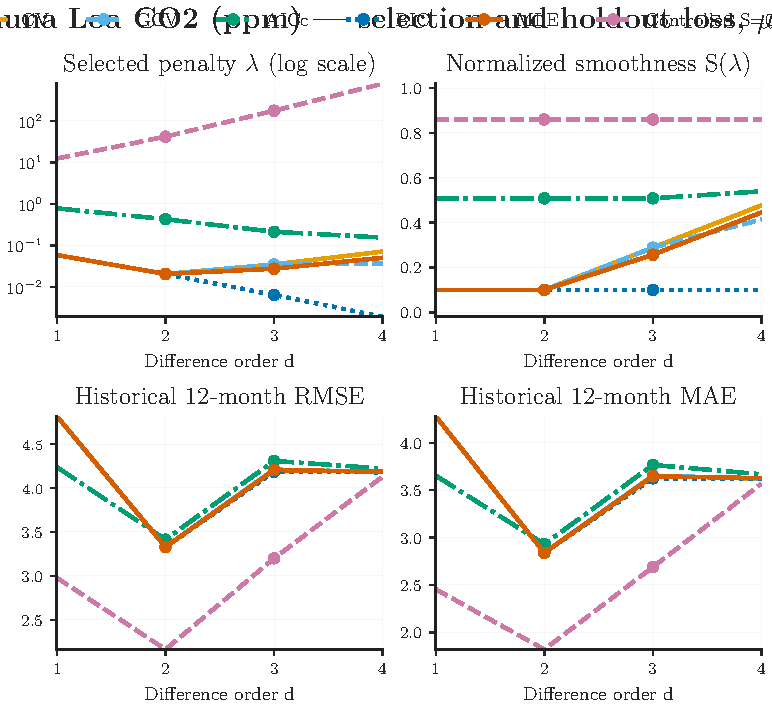
\includegraphics[width=\linewidth]{figures/co2_full_selection_summary_mu_zero.pdf}
\caption{Mauna Loa CO$_2$ with $\mu=0$:
selected $\lambda$ (log scale), normalized $S$,
and 12-month holdout RMSE and MAE by differencing
order and selection method. These are descriptive
single-origin losses, not a test of a calibrated
future-data predictive distribution.}
\label{fig:co2-selection-dashboard}
\end{figure}

\begin{table}[tbp]
\centering
\caption{Mauna Loa CO$_2$: all six selection procedures
for $d=2$, showing fixed-zero versus data-derived
reference differences. These are one-origin
descriptive holdout losses (ppm). AICc, BIC,
CV, GCV and MLE select from the same finite
penalty grid; Controlled is prescribed.}
\label{tab:dashboard-summary}
\footnotesize
\begin{tabular}{llrrrrr}
\toprule
$\mu$ mode & Selector & $\mu$ & $\lambda$ & $S$ & RMSE & MAE \\
\midrule
$0$ fixed & CV & 0 & 0.0205 & 0.100 & 3.328 & 2.839 \\
$0$ fixed & GCV & 0 & 0.0205 & 0.100 & 3.328 & 2.839 \\
$0$ fixed & AICc & 0 & 0.428 & 0.509 & 3.413 & 2.930 \\
$0$ fixed & BIC & 0 & 0.0205 & 0.100 & 3.328 & 2.839 \\
$0$ fixed & MLE & 0 & 0.0205 & 0.100 & 3.328 & 2.839 \\
$0$ fixed & Controlled~S=0.86 & 0 & 41.8 & 0.860 & 2.162 & 1.820 \\
training plug-in & CV & -0.0062 & 0.0205 & 0.100 & 3.328 & 2.839 \\
training plug-in & GCV & -0.0062 & 0.0205 & 0.100 & 3.328 & 2.839 \\
training plug-in & AICc & -0.0062 & 0.428 & 0.509 & 3.414 & 2.931 \\
training plug-in & BIC & -0.0062 & 0.0205 & 0.100 & 3.328 & 2.839 \\
training plug-in & MLE & -0.0062 & 0.0205 & 0.100 & 3.328 & 2.839 \\
training plug-in & Controlled~S=0.86 & -0.0062 & 41.8 & 0.860 & 2.168 & 1.825 \\
\bottomrule
\end{tabular}

\end{table}

\subsection{Sensitivity to data-derived nonzero means}
The alternative reference mean must be estimated
separately for each $(d,\mathcal T)$ and thus can
alter fitted endpoints, selected smoothness,
and subsequent extrapolation. We compare the two
specifications without reusing a mean estimated on the
holdout observations.

\begin{figure}[p]
\centering
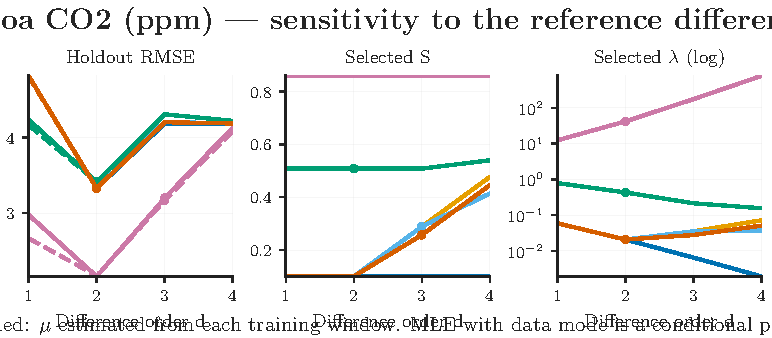
\includegraphics[width=\linewidth]{figures/co2_full_mu_sensitivity.pdf}
\caption{Mauna Loa CO$_2$: comparison of the
fixed $\mu=0$ (solid curves) and data-derived
$\mu$ (dashed) across $d$ for all six procedures.
Panels report historical holdout RMSE, selected
normalized smoothness and selected penalty.
The dashed results condition on the data-derived
reference difference mean, including for MLE;
they do not represent joint likelihood estimation
of $\mu$ and $\lambda$.}
\label{fig:co2-mu-sensitivity}
\end{figure}

\subsection{Economic-series comparison and supplementary figures}
The same complete factorial set of 24-panel dashboards
is reproduced for the US federal funds rate, and for
the last 120 months of Mauna Loa CO$_2$, with both
$\mu$ specifications. Figure~\ref{fig:fedfunds-holdout}
displays the economic-series holdout for $\mu=0$;
the remaining full-resolution PDF/SVG/PNG panels and
machine-readable per-cell results accompany the paper.

\begin{figure}[p]
\centering
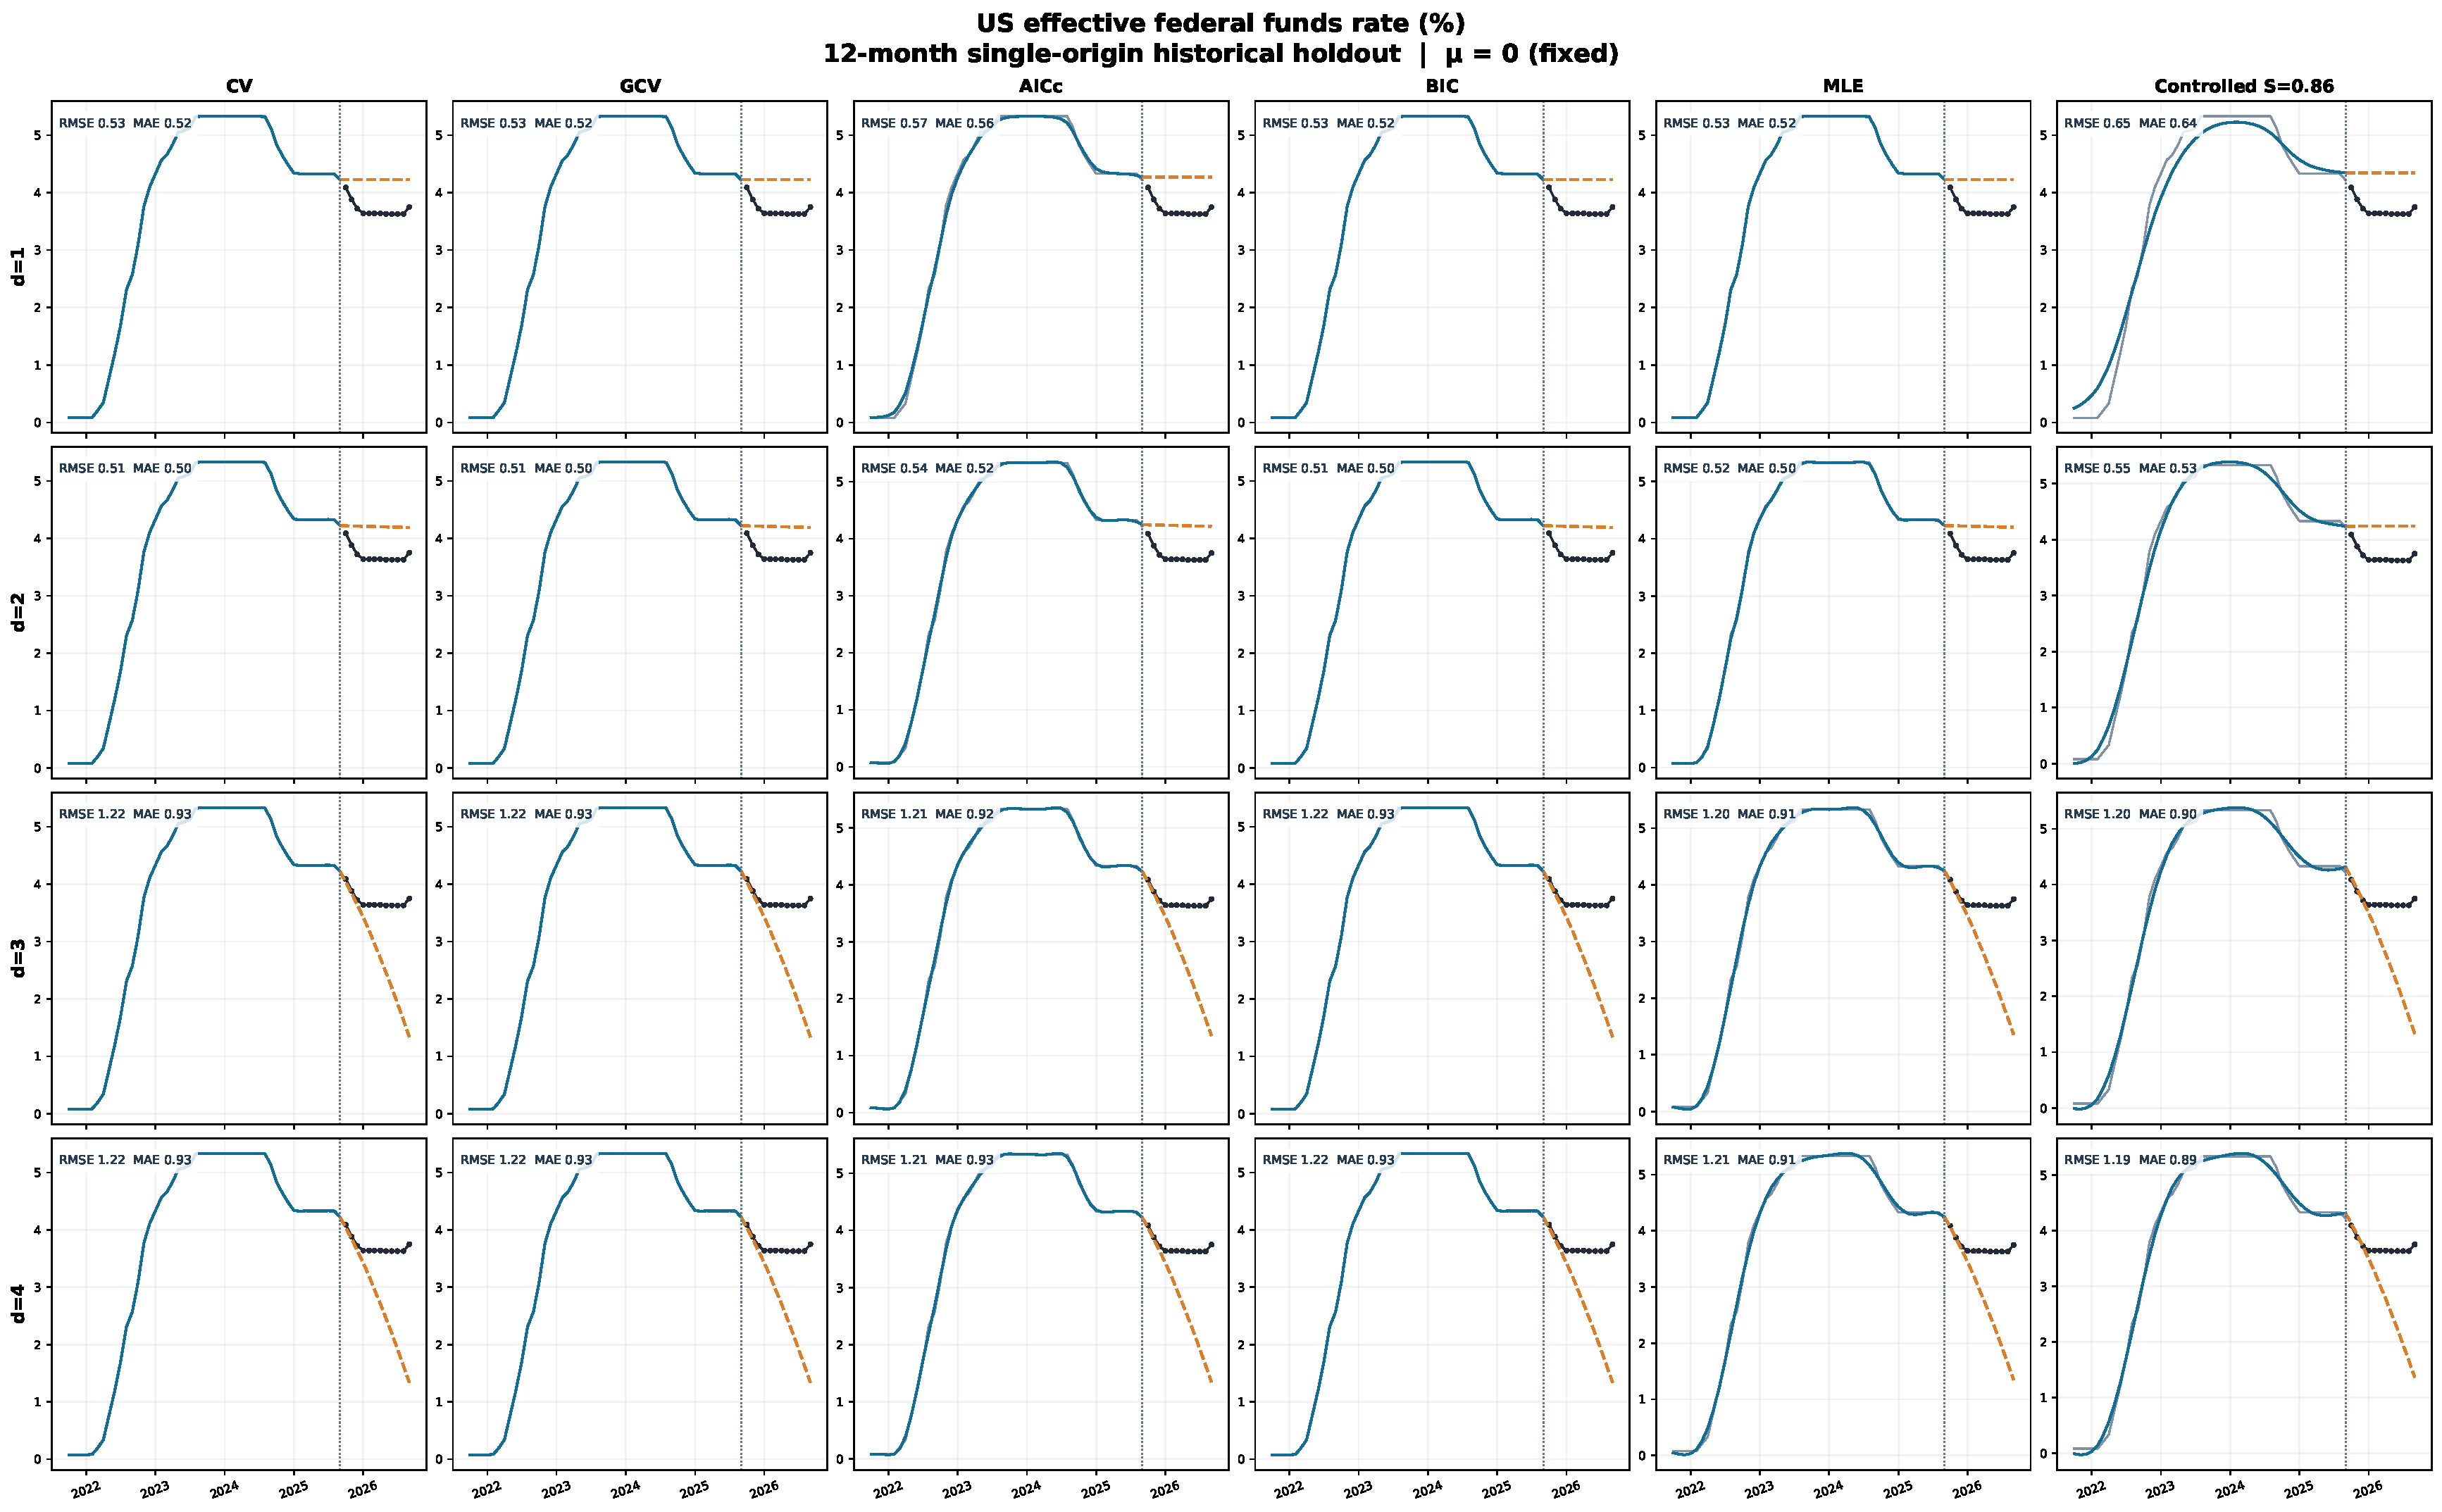
\includegraphics[width=\linewidth]{figures/fedfunds_full_dashboard_holdout_mu_zero.pdf}
\caption{Monthly US effective federal funds rate:
12-month historical holdout with $\mu=0$;
rows $d=1,2,3,4$, columns CV/GCV/AICc/BIC/MLE/
Controlled. The economic series is not seasonally
adjusted. The dashed segments are the same
anchored trend-extrapolation rule applied at the
training origin.}
\label{fig:fedfunds-holdout}
\end{figure}

A single held-out block, especially for CO$_2$ with
a pronounced annual cycle, cannot establish forecast
superiority; selection procedures target different
in-sample quantities and the extrapolation lacks a
seasonal model. For inferential forecasting claims,
further work requires multiple chronological origins,
horizon-specific evaluation, paired uncertainty
analysis, and explicit modelling of seasonal or
policy-driven changes. No optimization strategy here
is presented as universally superior solely because
of this illustration.
